\chapter{Contributions}

what made vgg ideal for ssds concept of detection on different scales was the gradual decrease in size of the feature map. We tried to mimic this behaviour by finding a suitably sized feature maps in other networks, which can complicate the implementation, especially in block architectures.


\section{Reimplement SSD on other base}
\subsection{ResNet-SSD}
\begin{figure}
    \resnetSSD
    \caption{SSD detector build on ResNet base. Depth of classification convolutions depends on number of classes (C). For detailed description of \textit{Layers} see \cref{fig:resnet_arch}.}
    \label{fig:resnetSSD}
\end{figure}

\subsection{Xception-SSD}


\begin{figure}
    \xceptionSSD
    \caption{SSD detector build on Xception base. Depth of classification convolutions depends on number of classes (C). Note that ReLU activation and batch normalization functions are omitted from this chart. For detailed description of blocks see \cref{fig:xception}}
    \label{fig:xceptionSSD}
\end{figure}


\subsection{Xception-B-SSD and Xception-C-SSD }

\begin{figure}
    \xceptionBSSD
    \caption{SSD detectors build on our modified Xception bases. We reduced the output depth of blocks 3 to 7 from 728 to 256 and as a consequence doubled the size of feature map. In version C, we also omitted blocks 5,6,7 and moved feature extraction from block 11 to block 10. For details on extra layers, classification and location layers see \cref{fig:xceptionSSD}}
    \label{fig:xceptionBSSD}
\end{figure}


\subsection{NasNet-SSD}

\begin{figure}
    \nasnetSSD
    \caption{SSD detector build on NASNet base. Depth of classification convolutions depends on number of classes (C). For detailed description of cells see \cref{sec:nasnet}}
    \label{fig:nasnetSSD}
\end{figure}


\subsection{Train results}
\begin{table}
    \begin{tabular}{c|c|c}
                            & coco      & small \\
        Resnet34-SSD        & 32.4      & 47.3  \\
        Resnet50-SSD        & 32.7      & 48.7  \\
        Resnet101-SSD       & 32.8      & 45.7  \\
        Xception-A-SSD      & 26.8      & 37.8  \\
        Xception-B-SSD      & -         & 48.4  \\
        Xception-C-SSD      & -         & x     \\
        NASNet-mobile-SSD   & -         & 36.9  \\
    \end{tabular}
    \caption{mean average precision, conf thr 0.2, IoU 0.5,  (400 epochs), 300x300 scaled random crops}
    \label{tab:map}
\end{table}

\begin{figure}
    \centering
    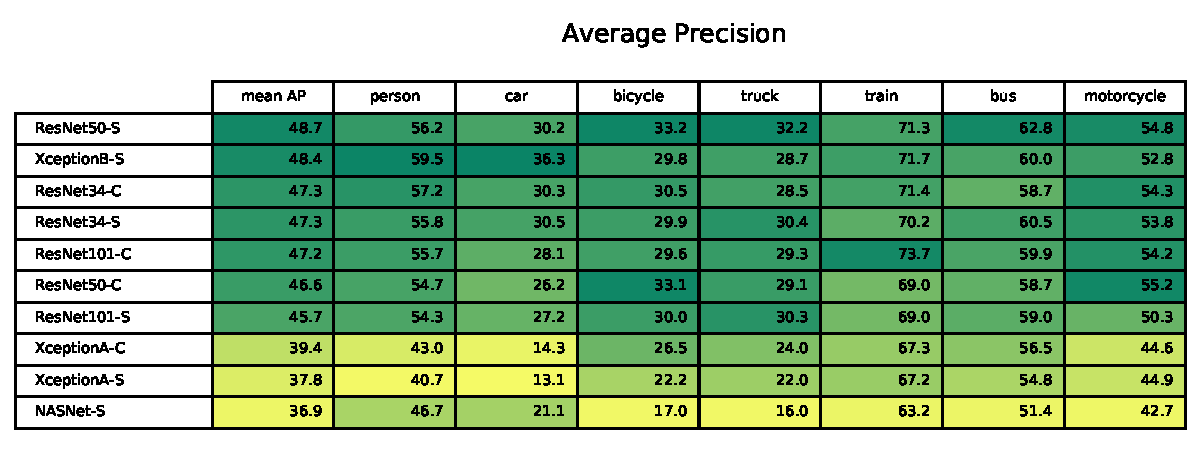
\includegraphics[width=\textwidth]{img/ap}
    \caption{AP, small 7 class dataset S, coco dataset C}
    \label{fig:ap}
\end{figure}


\begin{table}
    \begin{tabular}{c|c|c}
                    & 81cls     & 8cls  \\
    Resnet34        & 31.1M     & 24.4M \\
    Resnet50        & 45.5M     & 28.7M \\
    Resnet101       & 64.5M     & 47.7M \\
    Xception-A      & 40.6M     & 25.7M \\
    Xception-B      & x         & 19.2M \\
    Xception-C      & x         & xM    \\
    NASNet          & 17.3M     & 7.6M  \\
    VGG             & x         & 34.3M \\
    \end{tabular}
    \caption{total number of parameters}
    \label{tab:parameters}
\end{table}

fps
testing done on GTX 1080 Ti
10000 images, 300x300 
224x224 for nasnet
times include NMS


\section{something, use video continuity???}


